\thispagestyle{empty}

\newgeometry{tmargin=2cm, bmargin=2cm, lmargin=2cm, rmargin=2cm}

\section{Supplemental Figures and Tables}

\begin{figure*}[H]
	\begin{center}
	\centerline{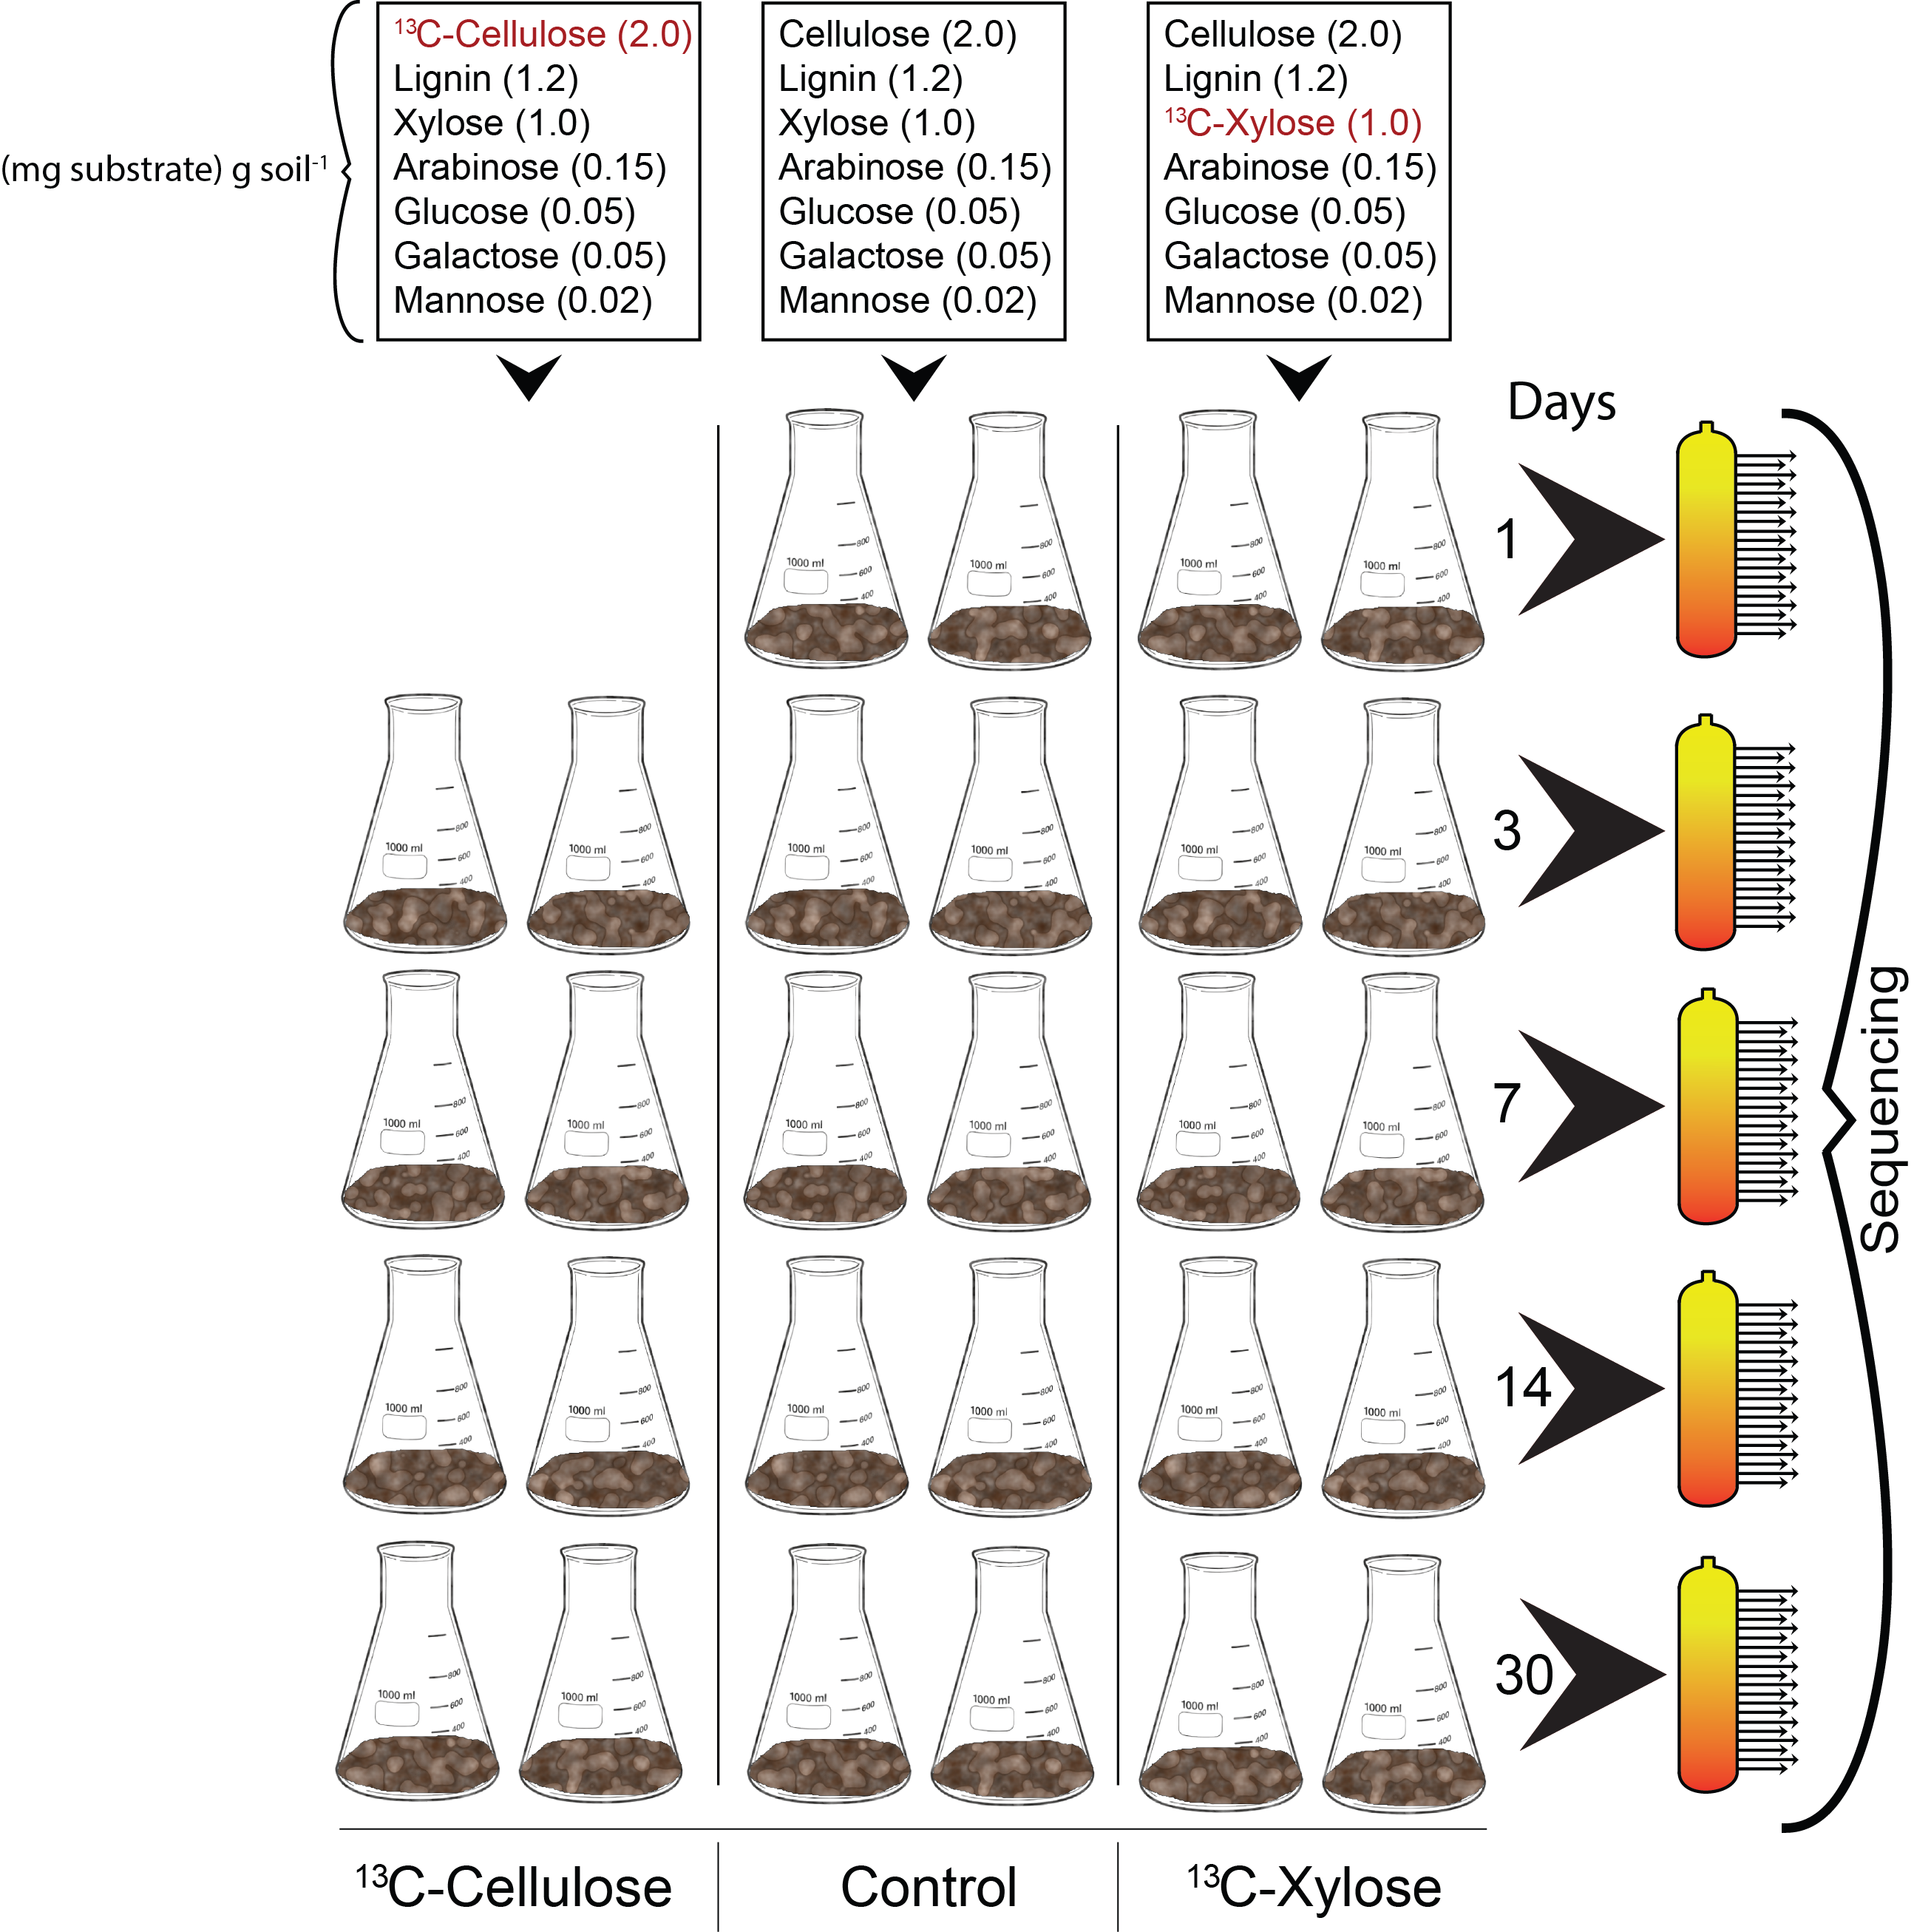
\includegraphics[width=0.75\textwidth]{figures/20150320methods_conceptual/20150320methods_conceptual.png}}
	\caption[Experimental Set Up]{\protectAn organic matter enrichment including C components and nutrients commonly found
in plant biomass was added to soil microcosms. At days
1, 3, 7, 14, and 30 replicate microcosms were destructively harvested. 
Bulk DNA from each treatment and time point
(n = 14) was subjected to CsCl density gradient centrifugation and density gradients
were fractionated (orange tubes wherein each arrow represents a fraction from the density gradient).
SSU rRNA genes were PCR amplified and sequenced from gradient fractions and
from non-fractionated DNA (representing the bulk soil microbial community).

}\label{fig:setup}
        \end{center}
\end{figure*}

\begin{figure*}[H]
	\begin{center}
	\centerline{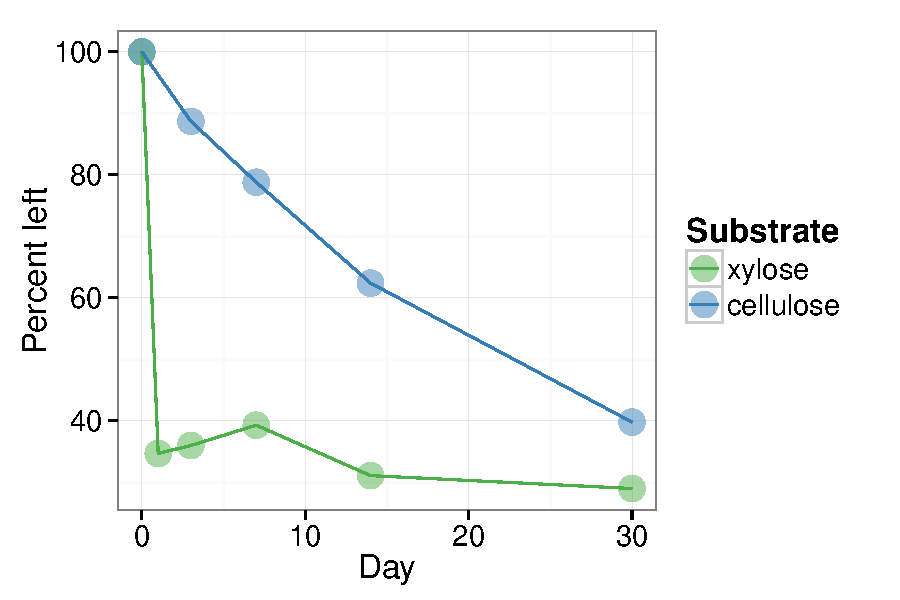
\includegraphics[width=11.4cm]{figures/13C_chart/13C_chart.pdf}}
	\caption{\protectPercentage of added $^{13}$C remaining in soil over time. C losses are likely
due to microbial respiration.
}\label{fig:13C}
        \end{center}
\end{figure*}

\begin{figure*}[H]
	\begin{center}
		\centerline{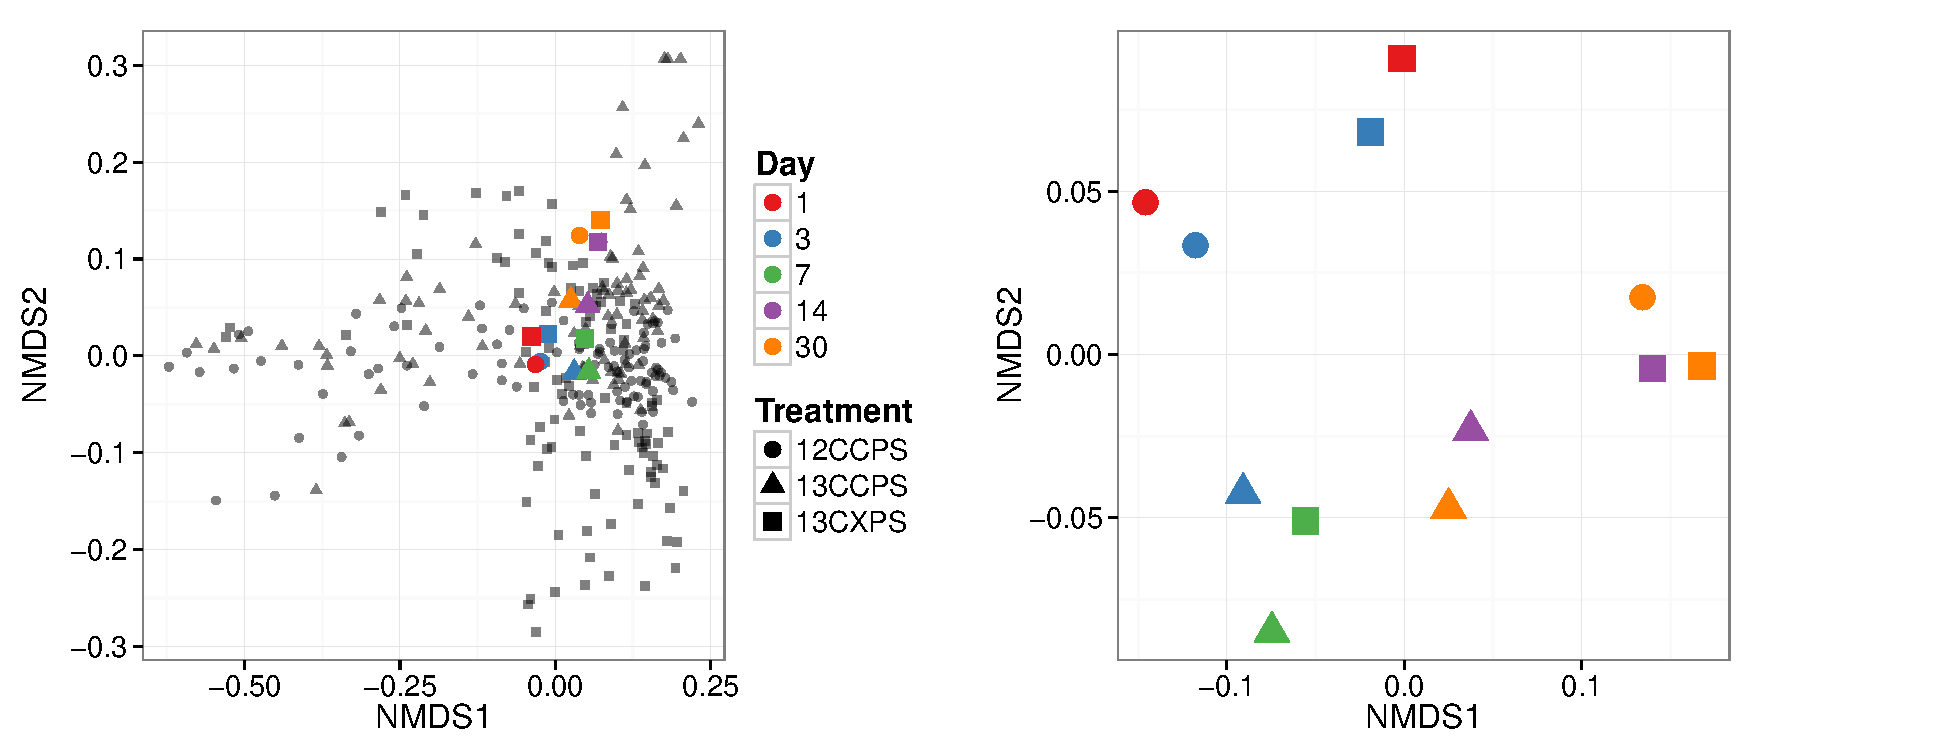
\includegraphics[width=\textwidth]{figures/bulk_ordination/bulk_ordination.pdf}}
	\caption[Ordination of bulk samples]{\protectNMDS analysis of SSU rRNA gene composition in non-fractionated DNA (colored points) indicates
that isotopic labelling does not alter overall microbial community composition,
microbial community composition in the soil microcosms changes over time, and
variance in non-fractionated DNA is smaller than variance in fractionated DNA (black points).
SSU rRNA gene sequences were determined for non-fractionated DNA from the
unlabeled control, $^{13}$C-xylose, and $^{13}$C-cellulose treatments over time (colors
indicate time, different symbols used for different treatments). Distance in SSU
rRNA gene composition was quantified with the UniFrac metric. The
leftmost panel indicates NMDS of data from both non-fractionated and
fractionated samples. The rightmost panel indicates NMDS of data only from
non-fractionated DNA. Statistical analysis is presented in main text.
}\label{fig:bulk_ord}
        \end{center}
\end{figure*}

\begin{figure*}[H] \begin{center}
\centerline{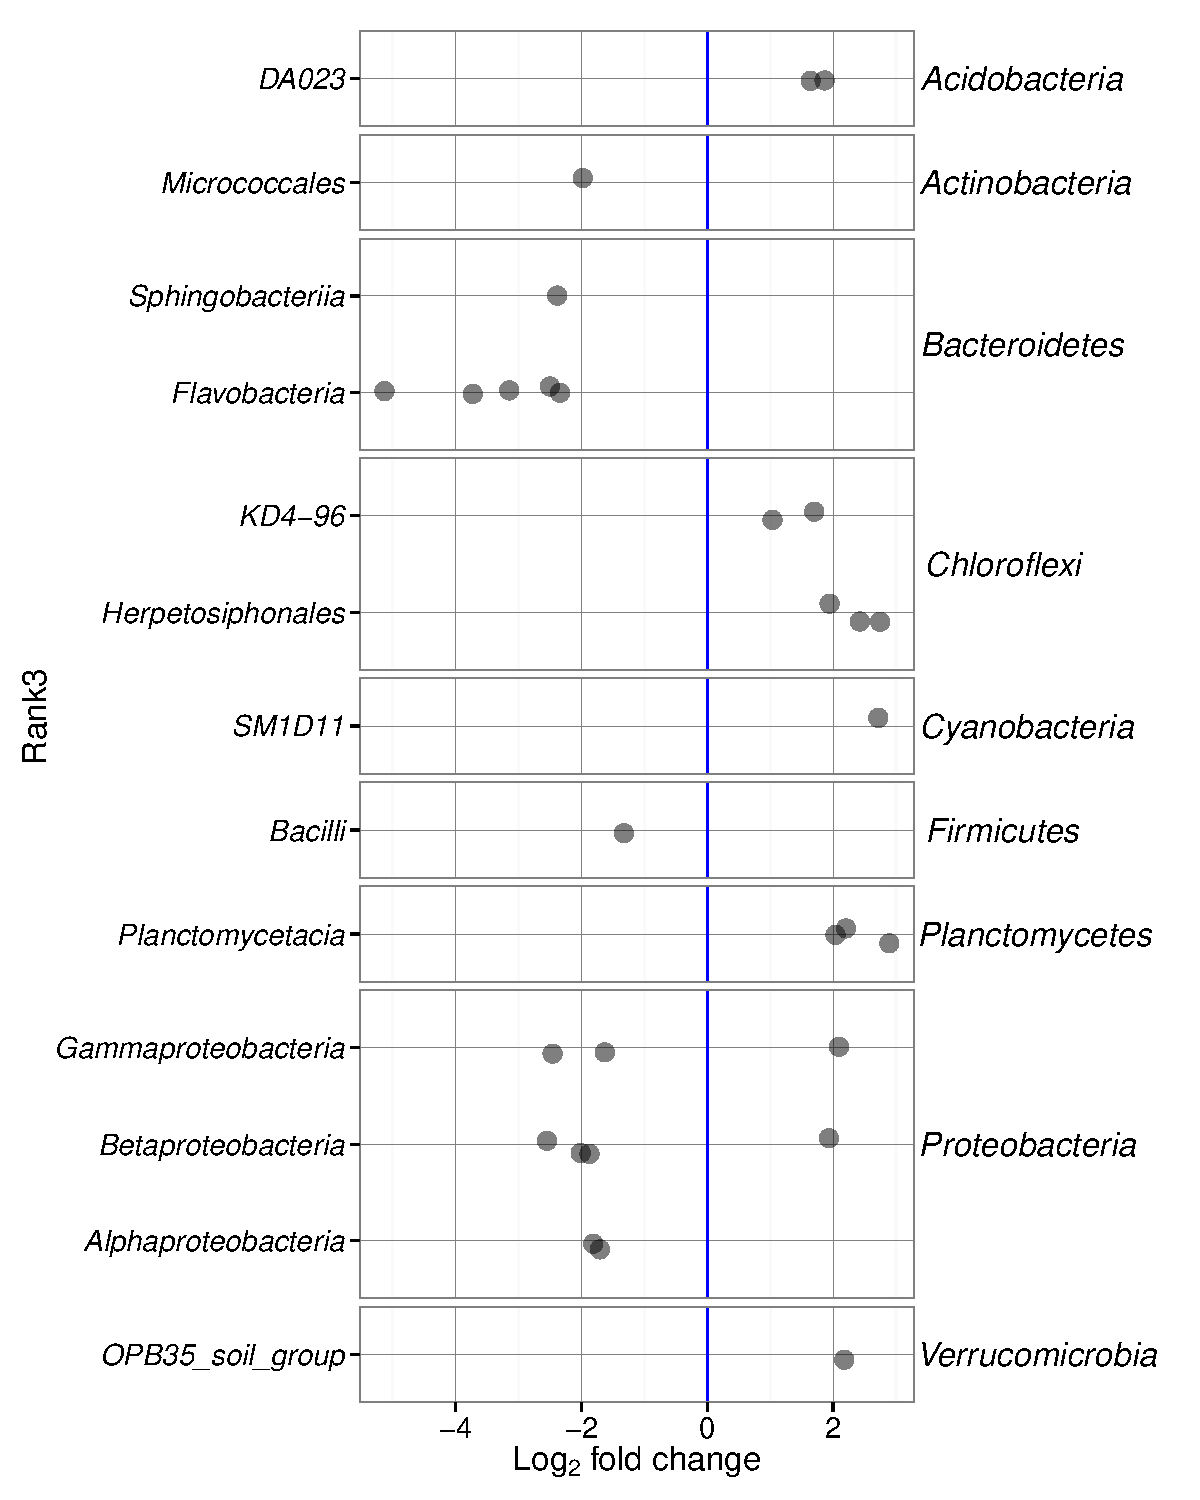
\includegraphics[width=0.75\textwidth]{figures/l2fc_time/l2fc_time.pdf}}
\caption[Temporal fluctuations for OTUs that changed significantly in abundance with time]{\protectFold change time$^{-1}$ for OTUs that changed significantly in abundance over time. One panel per phylum (phyla indicated on the right). Taxonomic class indicated on the left.}\label{fig:time}
\end{center} \end{figure*}

\begin{figure*}[H]
	\begin{center}
    \centerline{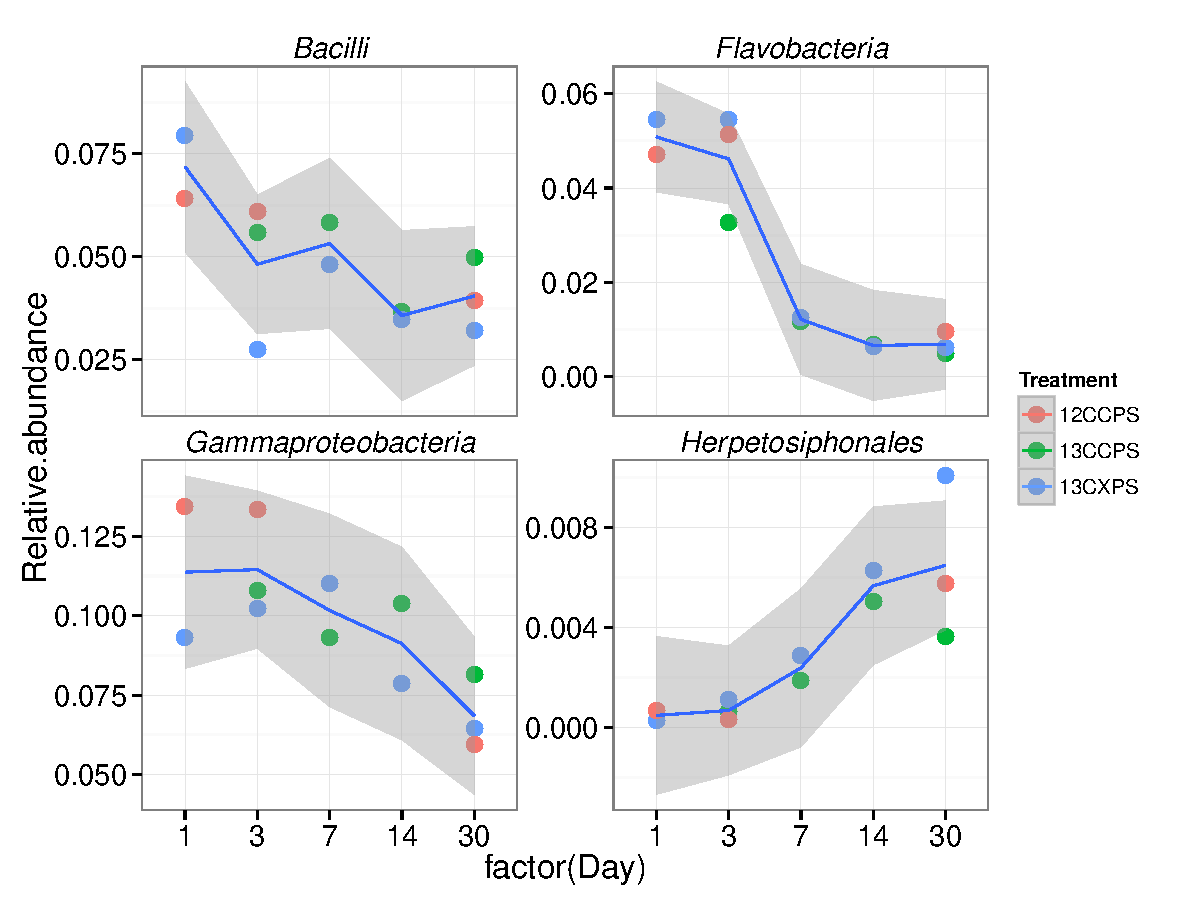
\includegraphics[width=0.85\textwidth]{figures/abndVtime_class/abndVtime_class.pdf}}
	\caption[Relative abundance of Classes over time for Classes that changed significantly in abundance with time]{\protectRelative abundance versus day for classes that changed significantly in relative abundance with time.}\label{fig:time_class}
    \end{center}
\end{figure*}

\begin{figure*}[H]
	\begin{center}
    \centerline{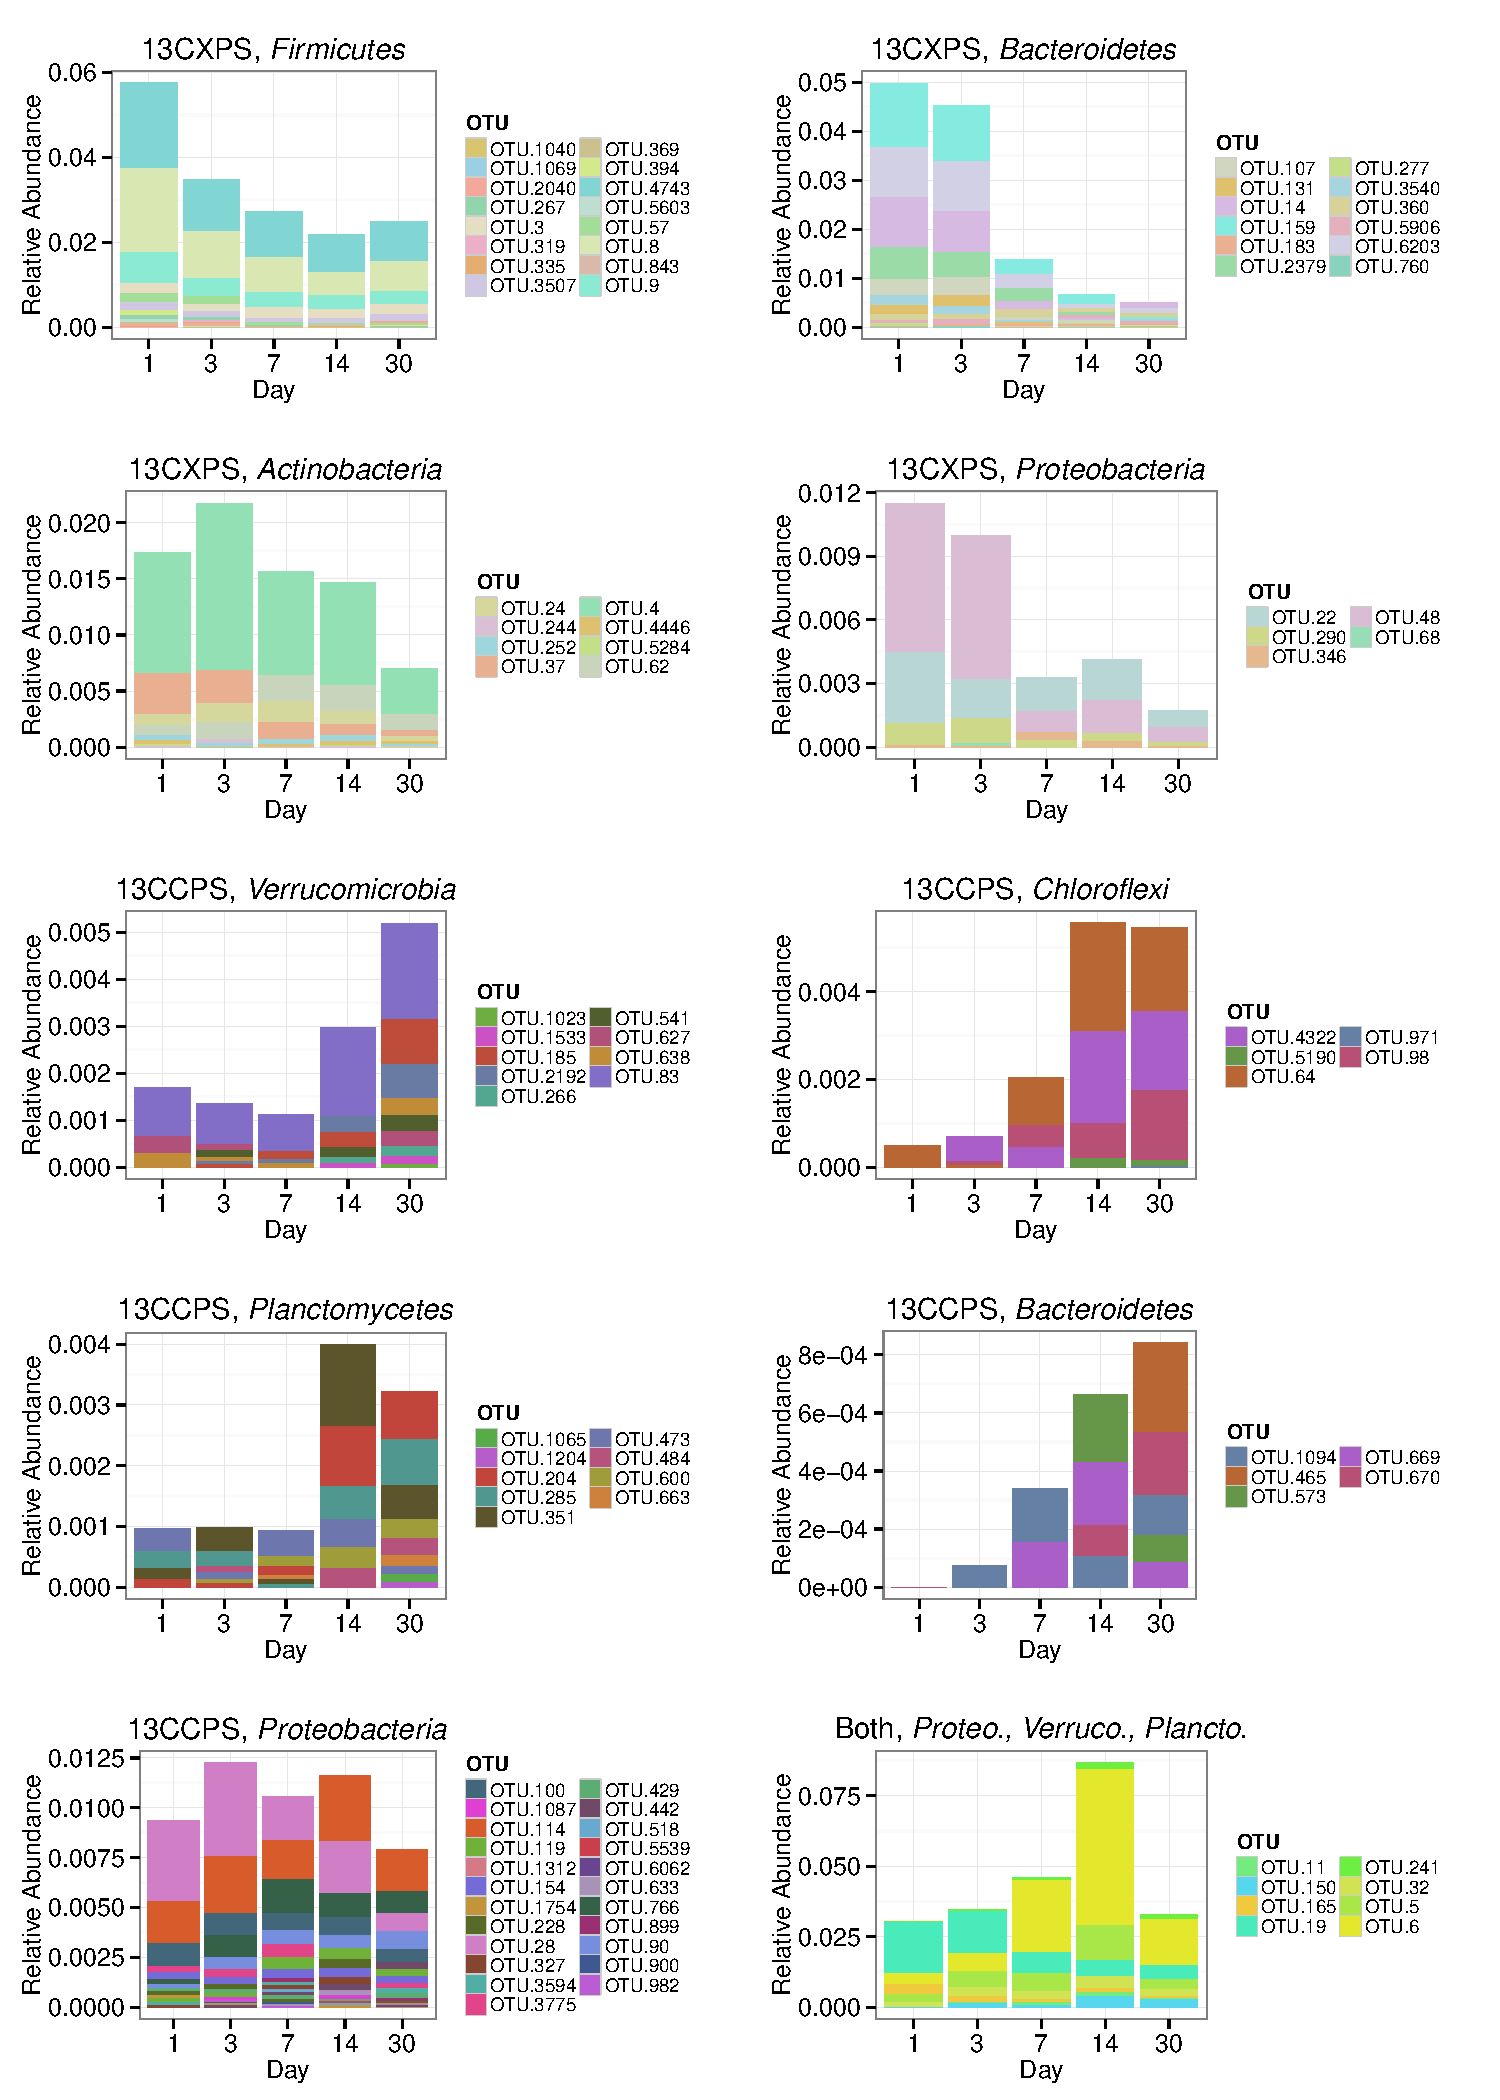
\includegraphics[width=0.75\textwidth]{figures/bulk_phylum_rspndr_abund/abund_v_time_phyla.pdf}}
	\caption{\protectChange in relative abundance in non-fractionated DNA over time for xylose
responders (13CXPS) and cellulose responders (13CCPS). Each panel represents
a phylum except for the lower right panel which shows all reponders to both
xylose and celluose. The abbreviations Proteo., Verruco., and Plancto.,
correspond to \textit{Proteobacteria}, \textit{Verrucomicrobia}, and \textit{Planctomycetes},
respectively.

}\label{fig:babund}
        \end{center}
\end{figure*}

\begin{figure*}[H]
	\begin{center}
    \centerline{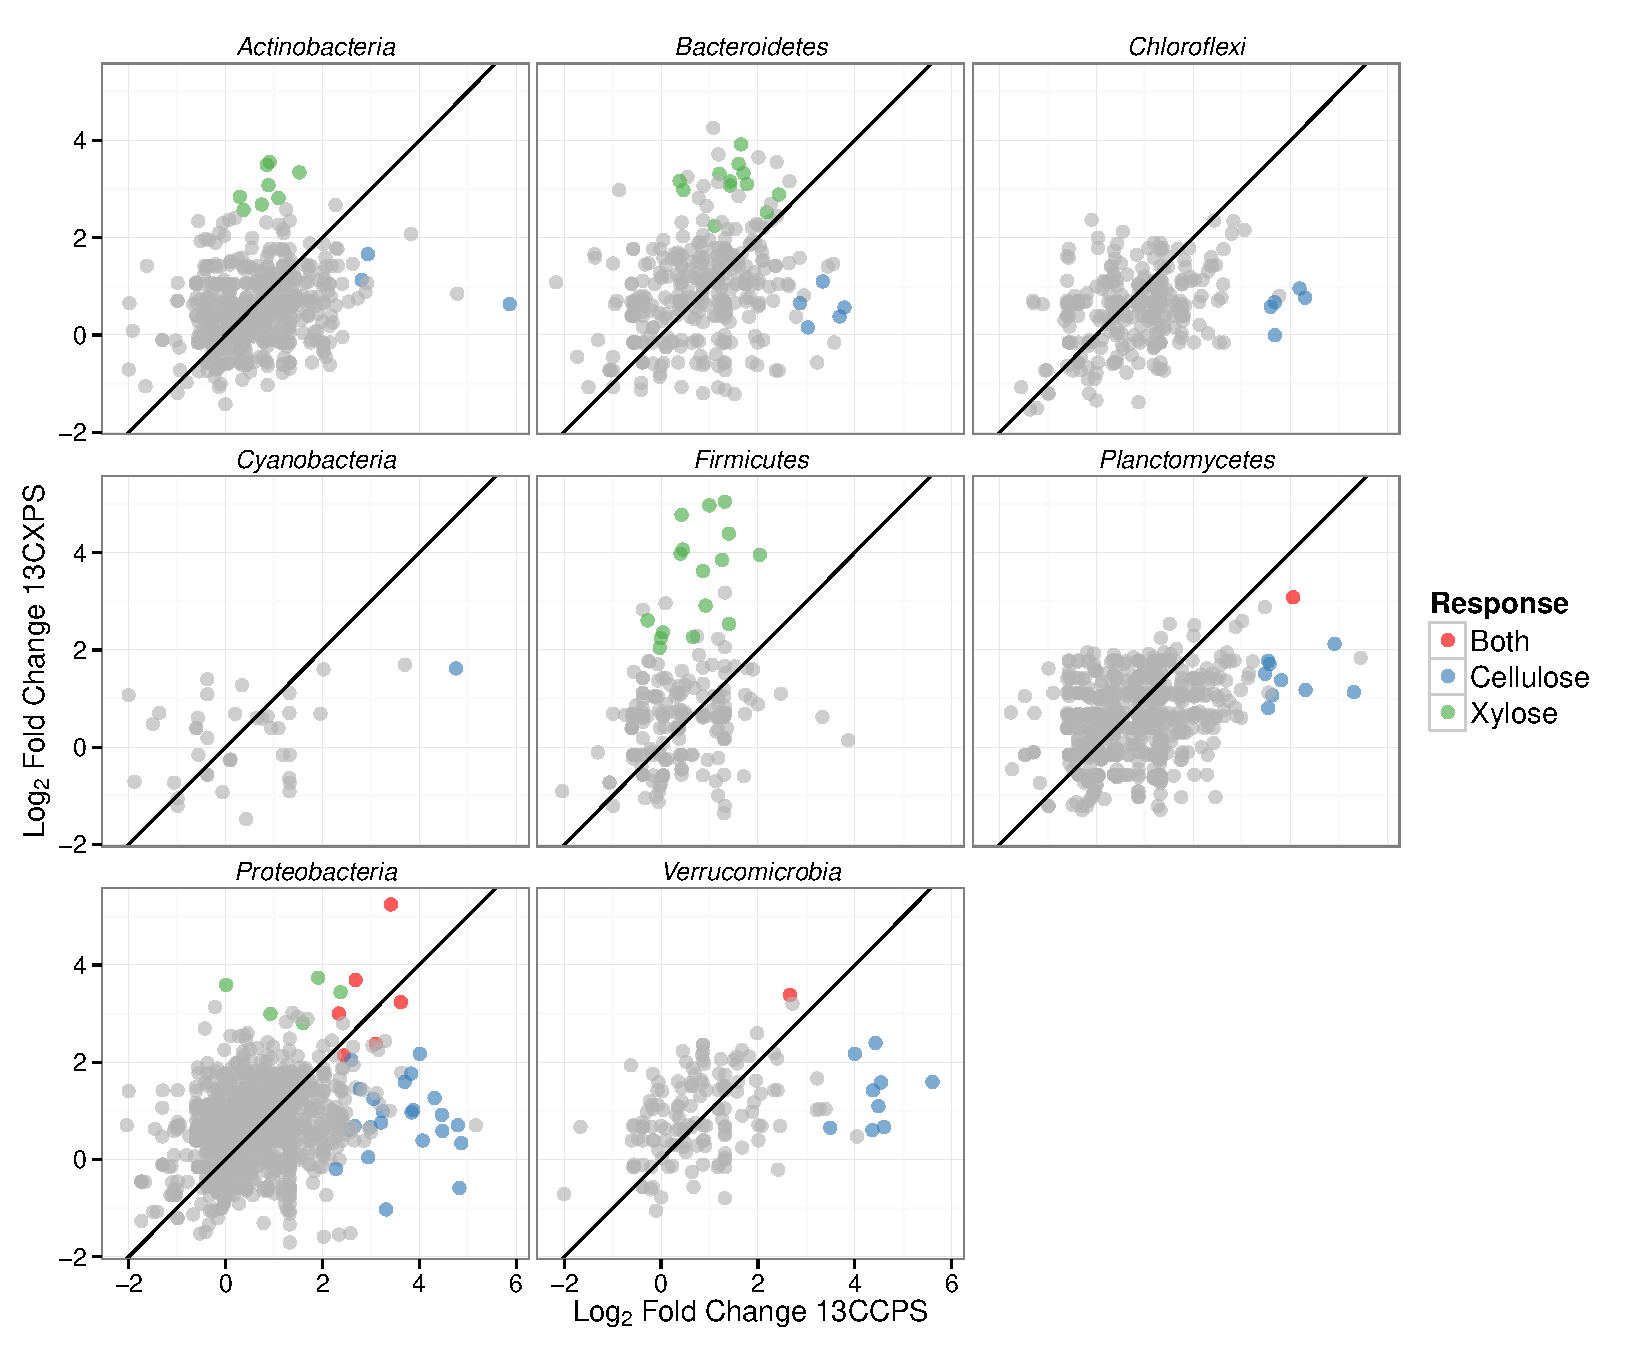
\includegraphics[width=11.4cm]{figures/generalist_specialist/generalist_specialist.pdf}}
    \caption{\protectMaximum enrichment at any point in time in heavy fractions of
$^{13}$C-treatments relative to controal (expressed as LFC) shown for
$^{13}$C-cellulose versus $^{13}$C-xylose treatments. Each point represents an
OTU. Blue points are cellulose responders, green xylose responders, and red are
responders to both xylose and cellulose, Grey points are OTUs that did not
repspond to either substrate. Line indicates a slope of one.
}\label{fig:genspec}
    \end{center} 
\end{figure*}

\begin{figure*}[H]
	\begin{center}
	\centerline{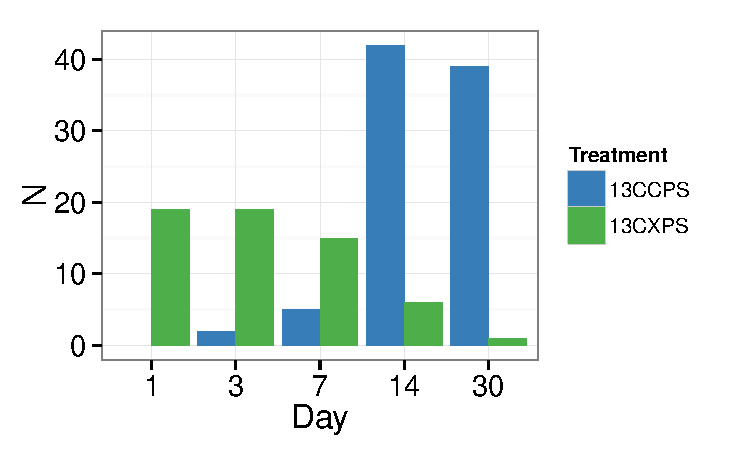
\includegraphics[width=0.75\textwidth]{figures/all_rspndr_bar/all_rspndr_bar.pdf}}
	\caption[Counts of $^{13}$C-responders at each day]{\protectCounts of responders to each isotopically labeled substrate (cellulose and xylose) over time.}\label{fig:rspndr_count}
        \end{center}
\end{figure*}

\begin{figure*}[H]
	\begin{center}
	\centerline{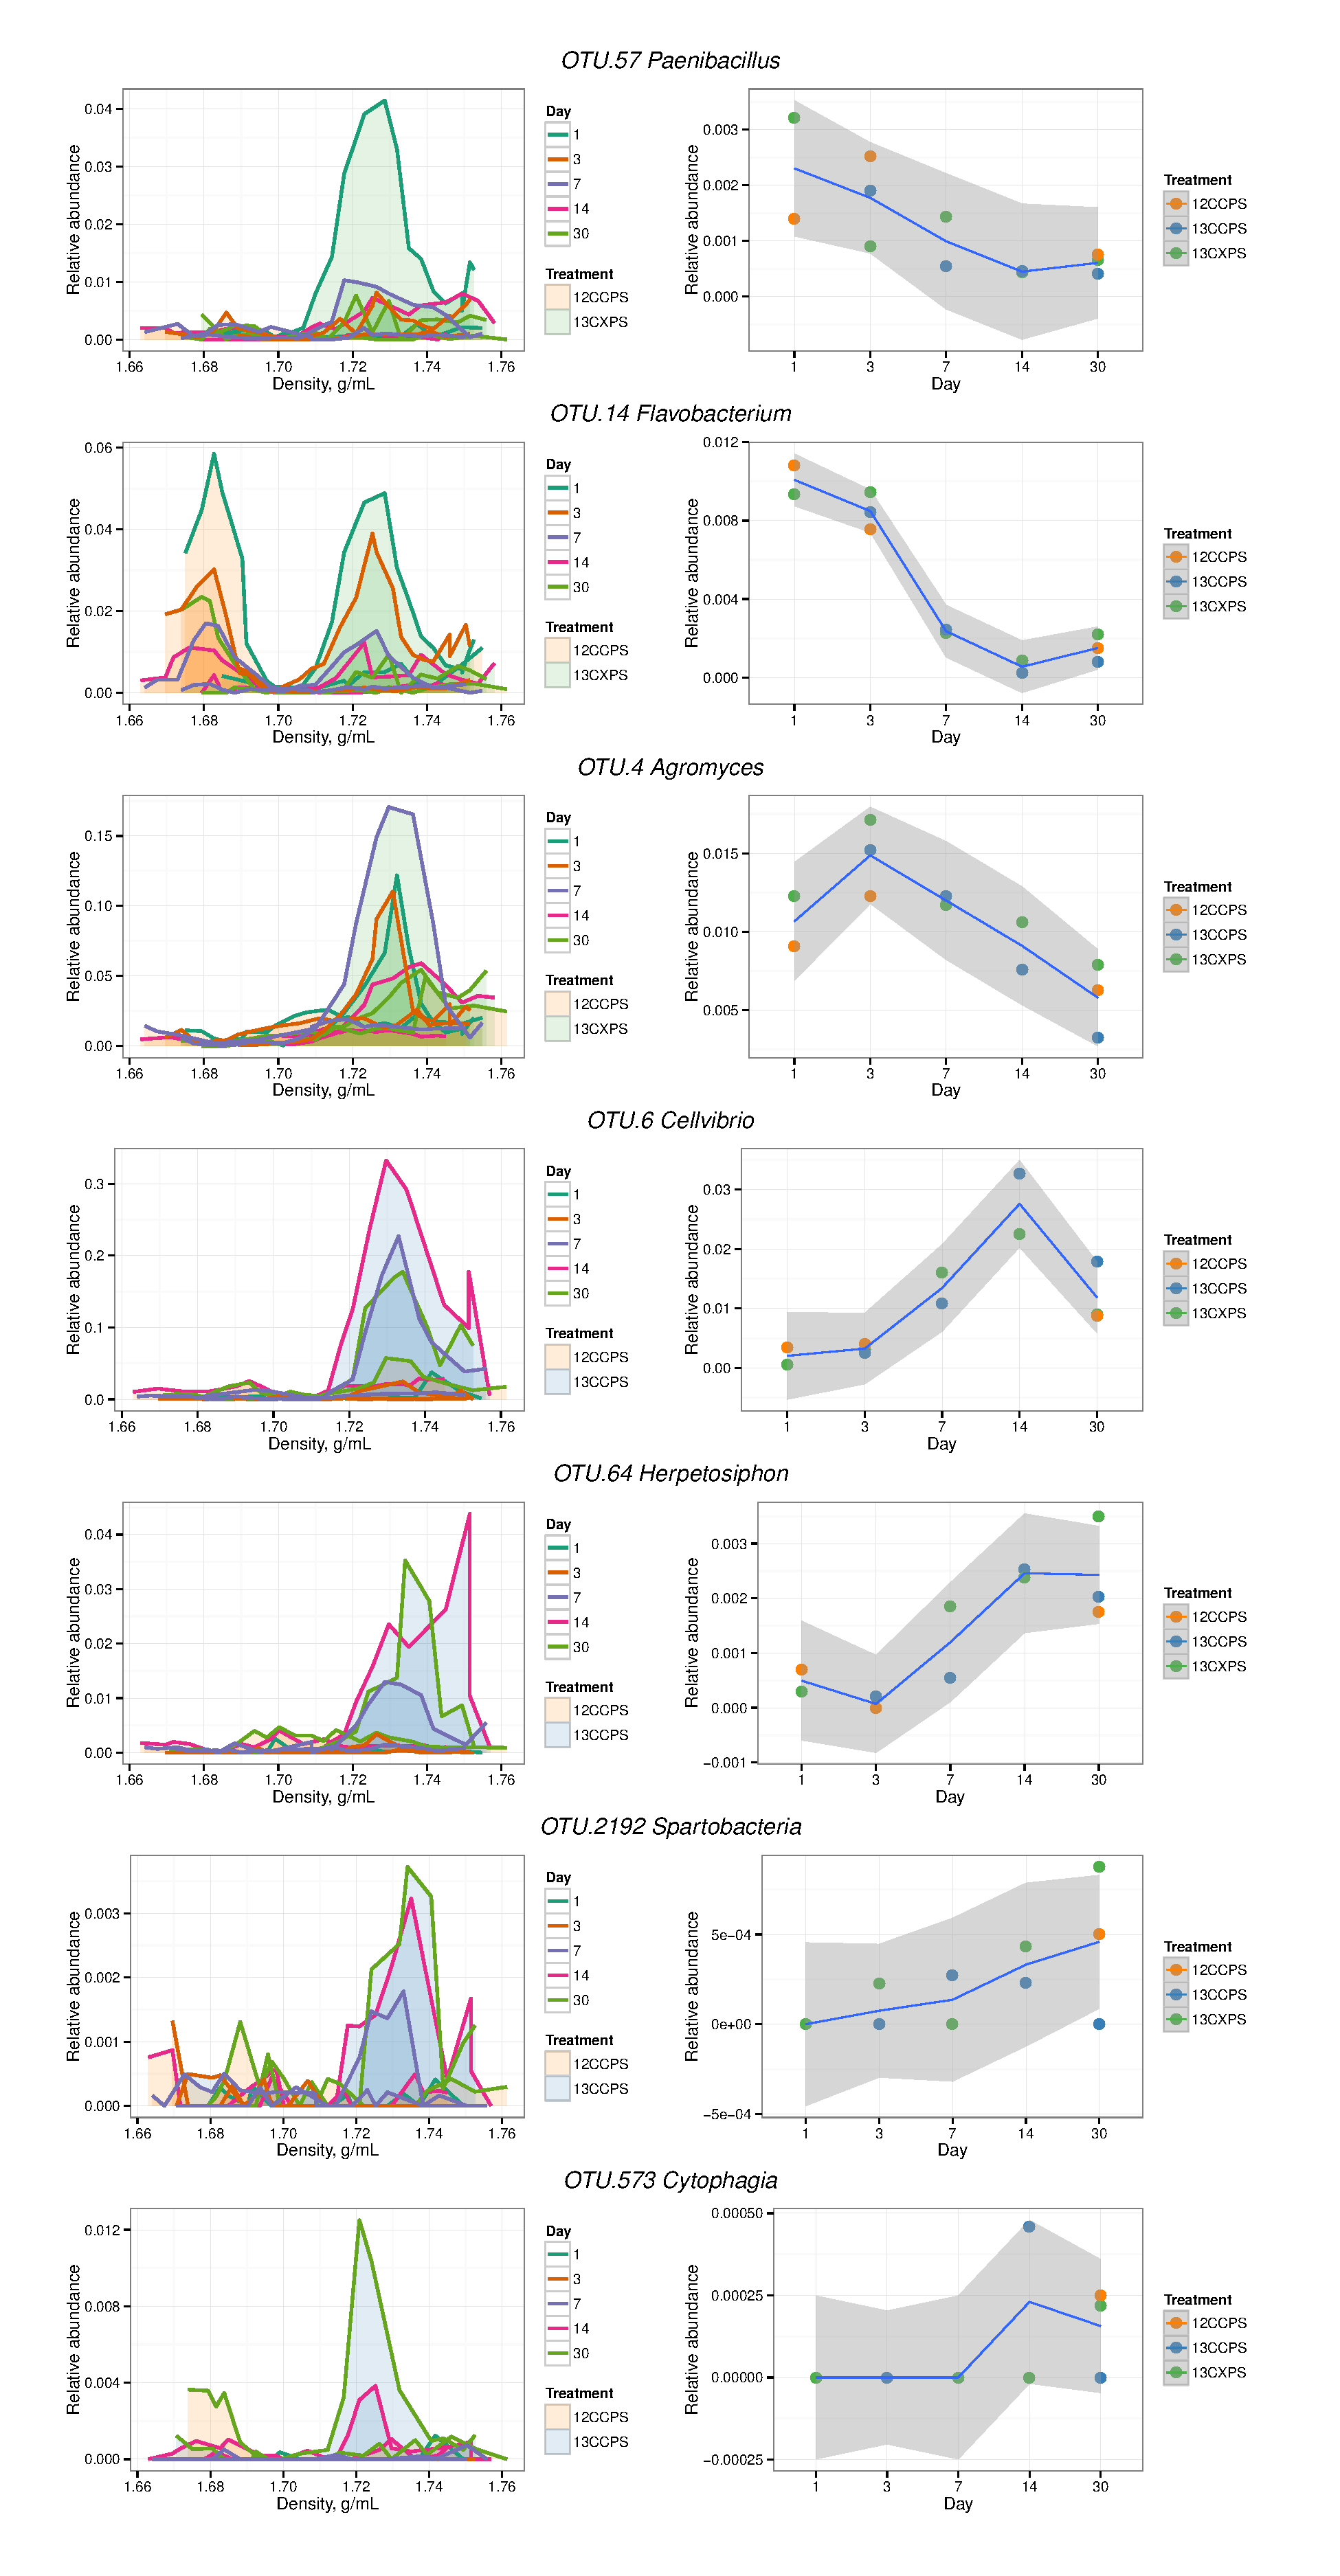
\includegraphics[width=0.65\textwidth]{figures/example/examples.pdf}}
	\caption[Counts of $^{13}$C-responders at each day]{\protectRaw data from example responders highlighted in the main text. The left column
shows DNA-SIP density fraction relative abundances for $^{13}$C-xylose or
$^{13}$C-cellulose gradients in addition to control gradients for each of the
chosen OTUs. Time is indicated by the color of the relative abundance profile
(see legend). Gradient profiles are shaded by treatment where orange represents
``control'' profles, blue ``$^{13}$C-cellulose'', and green
``$^{13}$C-xylose.'' The right column shows the relative abundance of each OTU
in non-fractionated DNA (i.e. the DNA that was subsequently fractionated on the
density gradient). Enrichment in the heavy end of the gradient in $^{13}$C
treatments indicates an OTU has $^{13}$C-labeled DNA that is greater in buoyant
density than it would be unlabeled.
}\label{fig:example}
        \end{center}
\end{figure*}

\begin{figure*}[H] \begin{center}
\centerline{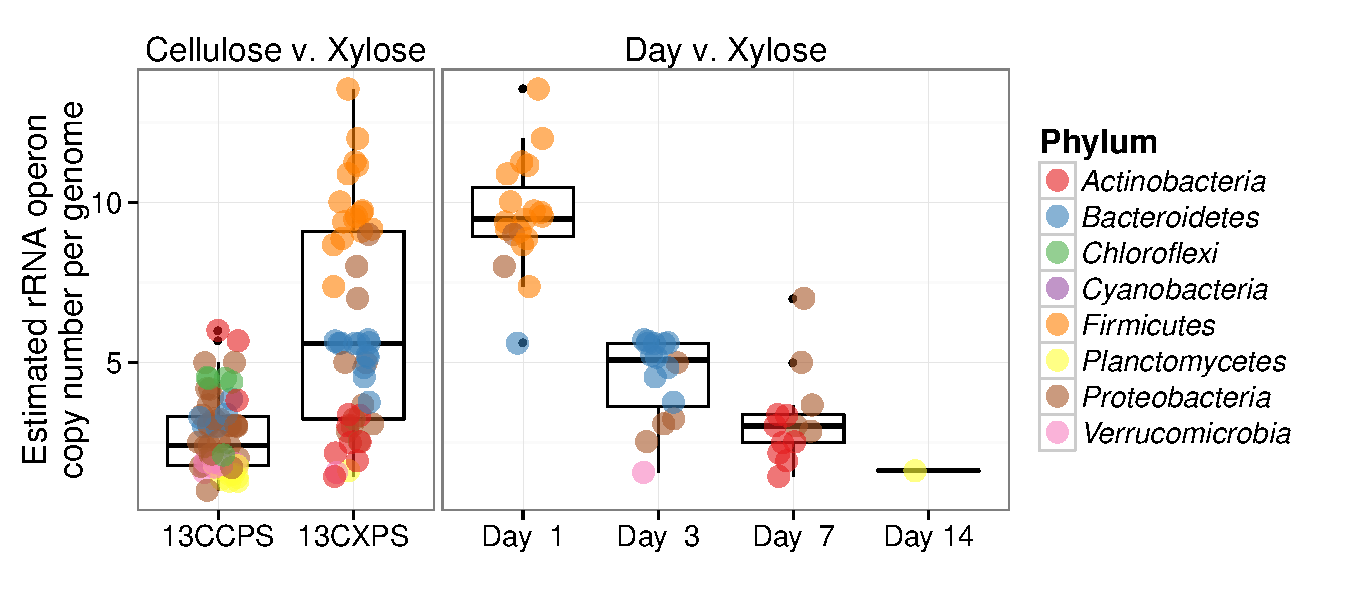
\includegraphics[width=\textwidth]{figures/copy_number/copy_number.pdf}}
\caption[OTU \textit{rrn} gene copy number with time and treatment]{\protectEstimated rRNA operon copy number for xylose and cellulose responders. The
leftmost panel contrasts estimated \textit{rrn} copy number for cellulose (13CCPS) and 
xylose (13CXPS) responders. The right panel shows estimated \textit{rrn} copy number
versus time of first response for xylose responders. Colors denote the phylum
of the OTUs (see legend).

}\label{fig:copy}
\end{center} \end{figure*}

\begin{figure*}[H] \begin{center}
\centerline{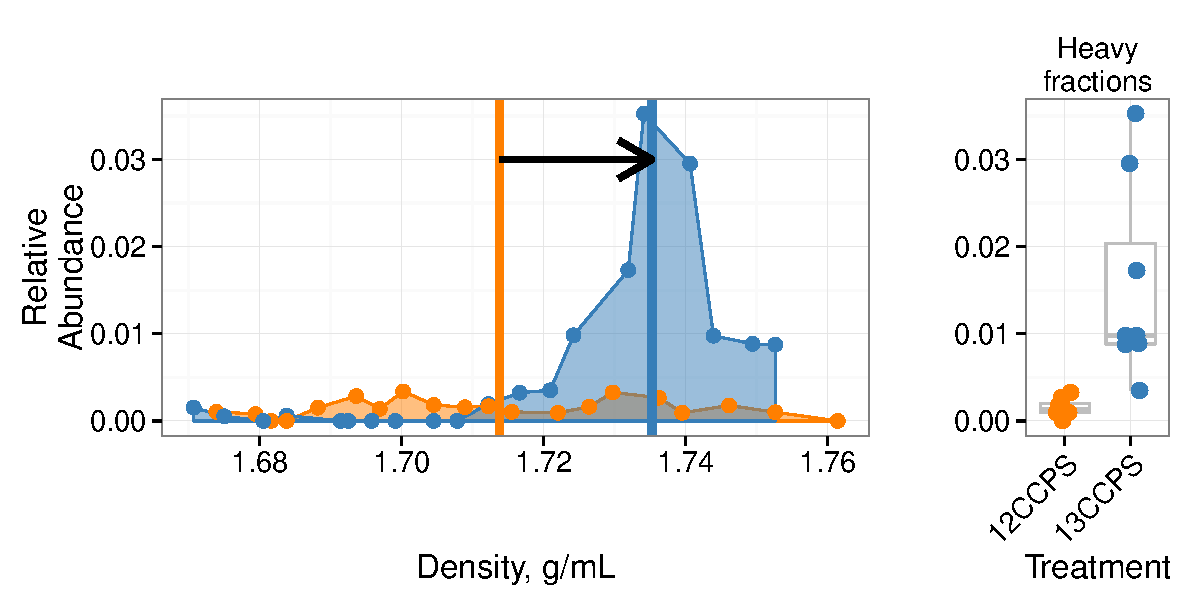
\includegraphics[width=0.75\textwidth]{figures/conceptual1/conceptual1.pdf}}
\caption[Density profile for an example "responder"]{\protectDensity profile for a single $^13$C-cellulose "responder" OTU in the labeled gradient, blue, and the control gradient, orange. Vertical lines show center of mass for each density profile and arrow denotes the magnitude and direction of the BD shift upon labeling. Panel at right shows relative abundance values in the heavy fractions for each gradient. }\label{fig:c1}
\end{center} \end{figure*}

\begin{figure*}[H] \begin{center}
\centerline{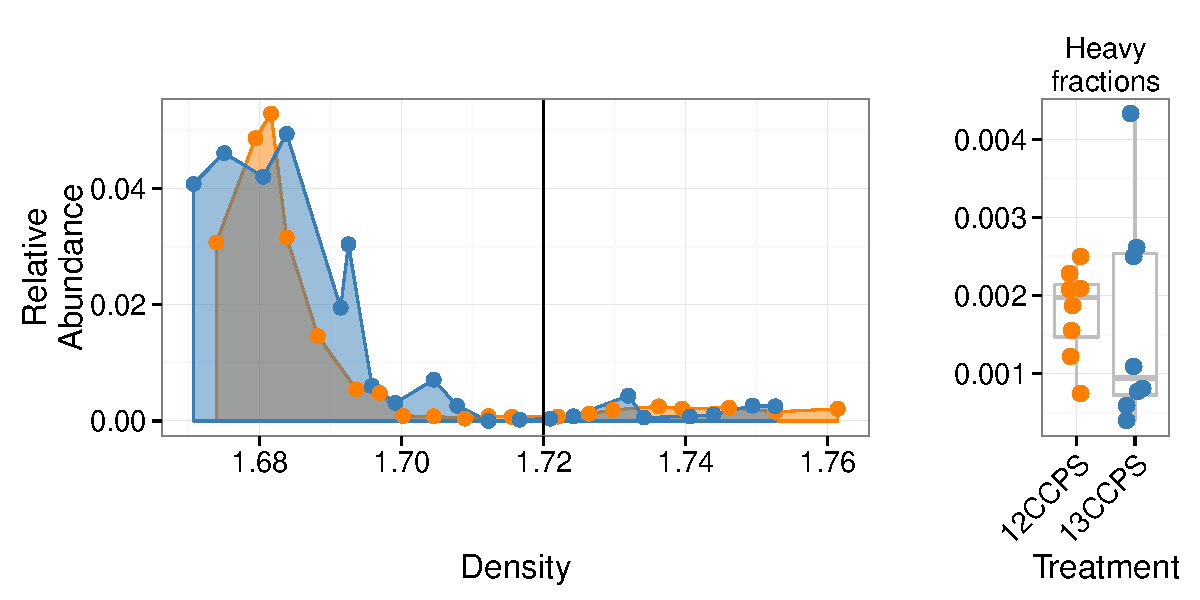
\includegraphics[width=0.75\textwidth]{figures/conceptual3/conceptual3.pdf}}
\caption[Density profile for example "non-responder"]{\protectDensity profile for a single non-responder OTU. The $^{13}$C-cellulose
treatment is in blue and the control treatment is in orange. The vertical line
shows where high density fractions begin as defined in our analysis. The right
panel shows relative abundance values in the high density fractions for each
gradient (The boxplot line is the median value. The box spans one
interquartile range (IR) about the median, whiskers extend 1.5 times the IR.  

}\label{fig:c3}
\end{center} \end{figure*}

%%%%%%%%%%%%%%%%%%%%%%%%%%%%%%%%%%%%%%%%%%%%%%%%%%%%%%%%%%%%%%%%%%%%%%%%%%%55%%%%%%

\begin{longtable}{lrp{5cm}rp{7cm}}

\caption{$^{13}$C-cellulose responders BLAST against Living Tree Project} \\
\toprule \\
    \textbf{OTU ID} & \textbf{Fold change} & \textbf{Top BLAST hits} & \textbf{BLAST \%ID} & \textbf{Phylum;Class;Order} \\
\midrule
\endfirsthead

\multicolumn{3}{c}
{{\tablename\ \thetable{} -- continued from previous page}} \\
\midrule
    \textbf{OTU ID} & \textbf{Fold change} & \textbf{Top BLAST hits} & \textbf{BLAST \%ID} & \textbf{Phylum;Class;Order} \\
\midrule
\endhead
    OTU.862 & 5.87 & \mbox{\textit{Allokutzneria albata}} & 100.0 & \mbox{\textit{Actinobacteria}} \mbox{\textit{Pseudonocardiales}} \mbox{\textit{Pseudonocardiaceae}} \\ \midrule
OTU.257 & 2.94 & \mbox{\textit{Lentzea waywayandensis}}, \mbox{\textit{Lentzea flaviverrucosa}} & 100.0 & \mbox{\textit{Actinobacteria}} \mbox{\textit{Pseudonocardiales}} \mbox{\textit{Pseudonocardiaceae}} \\ \midrule
OTU.132 & 2.81 & \mbox{\textit{Streptomyces spp.}} & 100.0 & \mbox{\textit{Actinobacteria}} \mbox{\textit{Streptomycetales}} \mbox{\textit{Streptomycetaceae}} \\ \midrule
OTU.465 & 3.79 & \mbox{\textit{Ohtaekwangia kribbensis}} & 92.73 & \mbox{\textit{Bacteroidetes}} \mbox{\textit{Cytophagia}} \mbox{\textit{Cytophagales}} \\ \midrule
OTU.1094 & 3.69 & \mbox{\textit{Sporocytophaga myxococcoides}} & 99.55 & \mbox{\textit{Bacteroidetes}} \mbox{\textit{Cytophagia}} \mbox{\textit{Cytophagales}} \\ \midrule
OTU.669 & 3.34 & \mbox{\textit{Ohtaekwangia koreensis}} & 92.69 & \mbox{\textit{Bacteroidetes}} \mbox{\textit{Cytophagia}} \mbox{\textit{Cytophagales}} \\ \midrule
OTU.573 & 3.03 & \mbox{\textit{Adhaeribacter aerophilus}} & 92.76 & \mbox{\textit{Bacteroidetes}} \mbox{\textit{Cytophagia}} \mbox{\textit{Cytophagales}} \\ \midrule
OTU.670 & 2.87 & \mbox{\textit{Adhaeribacter aerophilus}} & 91.78 & \mbox{\textit{Bacteroidetes}} \mbox{\textit{Cytophagia}} \mbox{\textit{Cytophagales}} \\ \midrule
OTU.971 & 3.68 & {No hits of at least 90\% identity} & 78.57 & \mbox{\textit{Chloroflexi}} \mbox{\textit{Anaerolineae}} \mbox{\textit{Anaerolineales}} \\ \midrule
OTU.64 & 4.31 & {No hits of at least 90\% identity} & 89.5 & \mbox{\textit{Chloroflexi}} \mbox{\textit{Herpetosiphonales}} \mbox{\textit{Herpetosiphonaceae}} \\ \midrule
OTU.4322 & 4.19 & {No hits of at least 90\% identity} & 89.14 & \mbox{\textit{Chloroflexi}} \mbox{\textit{Herpetosiphonales}} \mbox{\textit{Herpetosiphonaceae}} \\ \midrule
OTU.98 & 3.68 & {No hits of at least 90\% identity} & 88.18 & \mbox{\textit{Chloroflexi}} \mbox{\textit{Herpetosiphonales}} \mbox{\textit{Herpetosiphonaceae}} \\ \midrule
OTU.5190 & 3.6 & {No hits of at least 90\% identity} & 88.13 & \mbox{\textit{Chloroflexi}} \mbox{\textit{Herpetosiphonales}} \mbox{\textit{Herpetosiphonaceae}} \\ \midrule
OTU.120 & 4.76 & \mbox{\textit{Vampirovibrio chlorellavorus}} & 94.52 & \mbox{\textit{Cyanobacteria}} \mbox{\textit{SM1D11}} \mbox{\textit{uncultured-bacterium}} \\ \midrule
OTU.1065 & 5.31 & {No hits of at least 90\% identity} & 84.55 & \mbox{\textit{Planctomycetes}} \mbox{\textit{Planctomycetacia}} \mbox{\textit{Planctomycetales}} \\ \midrule
OTU.484 & 4.92 & {No hits of at least 90\% identity} & 89.09 & \mbox{\textit{Planctomycetes}} \mbox{\textit{Planctomycetacia}} \mbox{\textit{Planctomycetales}} \\ \midrule
OTU.1204 & 4.32 & \mbox{\textit{Planctomyces limnophilus}} & 91.78 & \mbox{\textit{Planctomycetes}} \mbox{\textit{Planctomycetacia}} \mbox{\textit{Planctomycetales}} \\ \midrule
OTU.150 & 4.06 & {No hits of at least 90\% identity} & 86.76 & \mbox{\textit{Planctomycetes}} \mbox{\textit{Planctomycetacia}} \mbox{\textit{Planctomycetales}} \\ \midrule
OTU.663 & 3.63 & \mbox{\textit{Pirellula staleyi DSM 6068}} & 90.87 & \mbox{\textit{Planctomycetes}} \mbox{\textit{Planctomycetacia}} \mbox{\textit{Planctomycetales}} \\ \midrule
OTU.473 & 3.58 & \mbox{\textit{Pirellula staleyi DSM 6068}} & 90.91 & \mbox{\textit{Planctomycetes}} \mbox{\textit{Planctomycetacia}} \mbox{\textit{Planctomycetales}} \\ \midrule
OTU.285 & 3.55 & \mbox{\textit{Blastopirellula marina}} & 90.87 & \mbox{\textit{Planctomycetes}} \mbox{\textit{Planctomycetacia}} \mbox{\textit{Planctomycetales}} \\ \midrule
OTU.351 & 3.54 & \mbox{\textit{Pirellula staleyi DSM 6068}} & 91.86 & \mbox{\textit{Planctomycetes}} \mbox{\textit{Planctomycetacia}} \mbox{\textit{Planctomycetales}} \\ \midrule
OTU.600 & 3.48 & {No hits of at least 90\% identity} & 80.37 & \mbox{\textit{Planctomycetes}} \mbox{\textit{Planctomycetacia}} \mbox{\textit{Planctomycetales}} \\ \midrule
OTU.900 & 4.87 & \mbox{\textit{Brevundimonas vesicularis}}, \mbox{\textit{Brevundimonas nasdae}} & 100.0 & \mbox{\textit{Proteobacteria}} \mbox{\textit{Alphaproteobacteria}} \mbox{\textit{Caulobacterales}} \\ \midrule
OTU.1754 & 4.48 & \mbox{\textit{Asticcacaulis biprosthecium}}, \mbox{\textit{Asticcacaulis benevestitus}} & 96.8 & \mbox{\textit{Proteobacteria}} \mbox{\textit{Alphaproteobacteria}} \mbox{\textit{Caulobacterales}} \\ \midrule
OTU.119 & 3.31 & \mbox{\textit{Brevundimonas alba}} & 100.0 & \mbox{\textit{Proteobacteria}} \mbox{\textit{Alphaproteobacteria}} \mbox{\textit{Caulobacterales}} \\ \midrule
OTU.327 & 2.99 & \mbox{\textit{Asticcacaulis biprosthecium}}, \mbox{\textit{Asticcacaulis benevestitus}} & 98.63 & \mbox{\textit{Proteobacteria}} \mbox{\textit{Alphaproteobacteria}} \mbox{\textit{Caulobacterales}} \\ \midrule
OTU.982 & 4.47 & \mbox{\textit{Devosia neptuniae}} & 100.0 & \mbox{\textit{Proteobacteria}} \mbox{\textit{Alphaproteobacteria}} \mbox{\textit{Rhizobiales}} \\ \midrule
OTU.1087 & 4.32 & \mbox{\textit{Devosia soli}}, \mbox{\textit{Devosia crocina}}, \mbox{\textit{Devosia riboflavina}} & 99.09 & \mbox{\textit{Proteobacteria}} \mbox{\textit{Alphaproteobacteria}} \mbox{\textit{Rhizobiales}} \\ \midrule
OTU.5539 & 4.01 & \mbox{\textit{Devosia subaequoris}} & 98.17 & \mbox{\textit{Proteobacteria}} \mbox{\textit{Alphaproteobacteria}} \mbox{\textit{Rhizobiales}} \\ \midrule
OTU.3775 & 3.88 & \mbox{\textit{Devosia glacialis}}, \mbox{\textit{Devosia chinhatensis}}, \mbox{\textit{Devosia geojensis}}, \mbox{\textit{Devosia yakushimensis}} & 98.63 & \mbox{\textit{Proteobacteria}} \mbox{\textit{Alphaproteobacteria}} \mbox{\textit{Rhizobiales}} \\ \midrule
OTU.429 & 3.7 & \mbox{\textit{Devosia limi}}, \mbox{\textit{Devosia psychrophila}} & 97.72 & \mbox{\textit{Proteobacteria}} \mbox{\textit{Alphaproteobacteria}} \mbox{\textit{Rhizobiales}} \\ \midrule
OTU.766 & 3.21 & \mbox{\textit{Devosia insulae}} & 99.54 & \mbox{\textit{Proteobacteria}} \mbox{\textit{Alphaproteobacteria}} \mbox{\textit{Rhizobiales}} \\ \midrule
OTU.165 & 3.1 & \mbox{\textit{Rhizobium spp.}} & 100.0 & \mbox{\textit{Proteobacteria}} \mbox{\textit{Alphaproteobacteria}} \mbox{\textit{Rhizobiales}} \\ \midrule
OTU.28 & 2.59 & \mbox{\textit{Rhizobium giardinii}}, \mbox{\textit{Rhizobium tubonense}}, \mbox{\textit{Rhizobium tibeticum}}, \mbox{\textit{Rhizobium mesoamericanum CCGE 501}}, \mbox{\textit{Rhizobium herbae}}, \mbox{\textit{Rhizobium endophyticum}} & 99.54 & \mbox{\textit{Proteobacteria}} \mbox{\textit{Alphaproteobacteria}} \mbox{\textit{Rhizobiales}} \\ \midrule
OTU.19 & 2.44 & \mbox{\textit{Rhizobium spp.}}, \mbox{\textit{Arthrobacter spp.}} & 99.54 & \mbox{\textit{Proteobacteria}} \mbox{\textit{Alphaproteobacteria}} \mbox{\textit{Rhizobiales}} \\ \midrule
OTU.90 & 2.94 & \mbox{\textit{Sphingopyxis panaciterrae}}, \mbox{\textit{Sphingopyxis chilensis}}, \mbox{\textit{Sphingopyxis sp. BZ30}}, \mbox{\textit{Sphingomonas sp.}} & 100.0 & \mbox{\textit{Proteobacteria}} \mbox{\textit{Alphaproteobacteria}} \mbox{\textit{Sphingomonadales}} \\ \midrule
OTU.518 & 4.8 & \mbox{\textit{Hydrogenophaga intermedia}} & 100.0 & \mbox{\textit{Proteobacteria}} \mbox{\textit{Betaproteobacteria}} \mbox{\textit{Burkholderiales}} \\ \midrule
OTU.1312 & 4.07 & \mbox{\textit{Paucimonas lemoignei}} & 99.54 & \mbox{\textit{Proteobacteria}} \mbox{\textit{Betaproteobacteria}} \mbox{\textit{Burkholderiales}} \\ \midrule
OTU.5 & 3.69 & \mbox{\textit{Delftia tsuruhatensis}}, \mbox{\textit{Delftia lacustris}} & 100.0 & \mbox{\textit{Proteobacteria}} \mbox{\textit{Betaproteobacteria}} \mbox{\textit{Burkholderiales}} \\ \midrule
OTU.114 & 2.78 & \mbox{\textit{Herbaspirillum sp. SUEMI03}}, \mbox{\textit{Herbaspirillum sp. SUEMI10}}, \mbox{\textit{Oxalicibacterium solurbis}}, \mbox{\textit{Herminiimonas fonticola}}, \mbox{\textit{Oxalicibacterium horti}} & 100.0 & \mbox{\textit{Proteobacteria}} \mbox{\textit{Betaproteobacteria}} \mbox{\textit{Burkholderiales}} \\ \midrule
OTU.633 & 3.84 & {No hits of at least 90\% identity} & 89.5 & \mbox{\textit{Proteobacteria}} \mbox{\textit{Deltaproteobacteria}} \mbox{\textit{Myxococcales}} \\ \midrule
OTU.3594 & 3.83 & \mbox{\textit{Chondromyces robustus}} & 90.41 & \mbox{\textit{Proteobacteria}} \mbox{\textit{Deltaproteobacteria}} \mbox{\textit{Myxococcales}} \\ \midrule
OTU.442 & 3.05 & \mbox{\textit{Chondromyces robustus}} & 92.24 & \mbox{\textit{Proteobacteria}} \mbox{\textit{Deltaproteobacteria}} \mbox{\textit{Myxococcales}} \\ \midrule
OTU.32 & 3.0 & \mbox{\textit{Sandaracinus amylolyticus}} & 94.98 & \mbox{\textit{Proteobacteria}} \mbox{\textit{Deltaproteobacteria}} \mbox{\textit{Myxococcales}} \\ \midrule
OTU.228 & 2.54 & \mbox{\textit{Sorangium cellulosum}} & 98.17 & \mbox{\textit{Proteobacteria}} \mbox{\textit{Deltaproteobacteria}} \mbox{\textit{Myxococcales}} \\ \midrule
OTU.899 & 2.28 & \mbox{\textit{Enhygromyxa salina}} & 97.72 & \mbox{\textit{Proteobacteria}} \mbox{\textit{Deltaproteobacteria}} \mbox{\textit{Myxococcales}} \\ \midrule
OTU.6 & 3.62 & \mbox{\textit{Cellvibrio fulvus}} & 100.0 & \mbox{\textit{Proteobacteria}} \mbox{\textit{Gammaproteobacteria}} \mbox{\textit{Pseudomonadales}} \\ \midrule
OTU.11 & 5.25 & \mbox{\textit{Stenotrophomonas pavanii}}, \mbox{\textit{Stenotrophomonas maltophilia}}, \mbox{\textit{Pseudomonas geniculata}} & 99.54 & \mbox{\textit{Proteobacteria}} \mbox{\textit{Gammaproteobacteria}} \mbox{\textit{Xanthomonadales}} \\ \midrule
OTU.6062 & 4.83 & \mbox{\textit{Dokdonella sp. DC-3}}, \mbox{\textit{Luteibacter rhizovicinus}} & 97.26 & \mbox{\textit{Proteobacteria}} \mbox{\textit{Gammaproteobacteria}} \mbox{\textit{Xanthomonadales}} \\ \midrule
OTU.154 & 3.24 & \mbox{\textit{Pseudoxanthomonas mexicana}}, \mbox{\textit{Pseudoxanthomonas japonensis}} & 100.0 & \mbox{\textit{Proteobacteria}} \mbox{\textit{Gammaproteobacteria}} \mbox{\textit{Xanthomonadales}} \\ \midrule
OTU.100 & 2.66 & \mbox{\textit{Pseudoxanthomonas sacheonensis}}, \mbox{\textit{Pseudoxanthomonas dokdonensis}} & 100.0 & \mbox{\textit{Proteobacteria}} \mbox{\textit{Gammaproteobacteria}} \mbox{\textit{Xanthomonadales}} \\ \midrule
OTU.1023 & 4.61 & {No hits of at least 90\% identity} & 80.54 & \mbox{\textit{Verrucomicrobia}} \mbox{\textit{Spartobacteria}} \mbox{\textit{Chthoniobacterales}} \\ \midrule
OTU.266 & 4.54 & {No hits of at least 90\% identity} & 83.64 & \mbox{\textit{Verrucomicrobia}} \mbox{\textit{Spartobacteria}} \mbox{\textit{Chthoniobacterales}} \\ \midrule
OTU.541 & 4.49 & {No hits of at least 90\% identity} & 84.23 & \mbox{\textit{Verrucomicrobia}} \mbox{\textit{Spartobacteria}} \mbox{\textit{Chthoniobacterales}} \\ \midrule
OTU.185 & 4.37 & {No hits of at least 90\% identity} & 85.14 & \mbox{\textit{Verrucomicrobia}} \mbox{\textit{Spartobacteria}} \mbox{\textit{Chthoniobacterales}} \\ \midrule
OTU.2192 & 3.49 & {No hits of at least 90\% identity} & 83.56 & \mbox{\textit{Verrucomicrobia}} \mbox{\textit{Spartobacteria}} \mbox{\textit{Chthoniobacterales}} \\ \midrule
OTU.1533 & 3.43 & {No hits of at least 90\% identity} & 82.27 & \mbox{\textit{Verrucomicrobia}} \mbox{\textit{Spartobacteria}} \mbox{\textit{Chthoniobacterales}} \\ \midrule
OTU.241 & 3.38 & {No hits of at least 90\% identity} & 87.73 & \mbox{\textit{Verrucomicrobia}} \mbox{\textit{Spartobacteria}} \mbox{\textit{Chthoniobacterales}} \\ \midrule
OTU.83 & 5.61 & \mbox{\textit{Luteolibacter sp. CCTCC AB 2010415}} & 97.72 & \mbox{\textit{Verrucomicrobia}} \mbox{\textit{Verrucomicrobiae}} \mbox{\textit{Verrucomicrobiales}} \\ \midrule
OTU.627 & 4.43 & \mbox{\textit{Verrucomicrobiaceae bacterium DC2a-G7}} & 100.0 & \mbox{\textit{Verrucomicrobia}} \mbox{\textit{Verrucomicrobiae}} \mbox{\textit{Verrucomicrobiales}} \\ \midrule
OTU.638 & 4.0 & \mbox{\textit{Luteolibacter sp. CCTCC AB 2010415}}, \mbox{\textit{Luteolibacter algae}} & 93.61 & \mbox{\textit{Verrucomicrobia}} \mbox{\textit{Verrucomicrobiae}} \mbox{\textit{Verrucomicrobiales}} \\ \midrule

\bottomrule
\label{tab:cell}
\end{longtable}

\thispagestyle{empty}
\newgeometry{tmargin=2cm, bmargin=2cm, lmargin=0.25cm, rmargin=0.25cm} 

\begin{ThreePartTable}
\begin{TableNotes}
\item[a] Maximum observed $log_{2}$ of fold change. 
\item[b] Day of maximum fold change.
\item[c] All response days.
\end{TableNotes}

\begin{longtable}{P{1.5cm}rP{1cm}P{1.5cm}P{4cm}rP{5cm}}

\caption{$^{13}$C-xylose responders BLAST against Living Tree Project} \\
\label{tab:xyl}
\toprule 
    \textbf{OTU ID} & 
    \textbf{Fold change} \tnote{a} & 
    \textbf{Day} \tnote{b} & 
    \textbf{All days} \tnote{c} &
    \textbf{Top BLAST hits} & 
    \textbf{BLAST \%ID} & 
    \textbf{Phylum;Class;Order} \\
\midrule
\endfirsthead

\multicolumn{3}{c}
{{\tablename\ \thetable{} -- continued from previous page}} \\
\midrule
    \textbf{OTU ID} & 
    \textbf{Fold change} & 
    \textbf{Day} & 
    \textbf{All days} &
    \textbf{Top BLAST hits} & 
    \textbf{BLAST \%ID} & 
    \textbf{Phylum;Class;Order} \\
\midrule
\endhead
    OTU.1040 & 4.78 & 1 & 1&\mbox{\textit{Paenibacillus daejeonensis}} & 100.0 & \mbox{\textit{Firmicutes}} \mbox{\textit{Bacilli}} \mbox{\textit{Bacillales}} \\ \midrule
OTU.1069 & 3.85 & 1 & 1&\mbox{\textit{Paenibacillus terrigena}} & 100.0 & \mbox{\textit{Firmicutes}} \mbox{\textit{Bacilli}} \mbox{\textit{Bacillales}} \\ \midrule
OTU.107 & 2.25 & 3 & 3&\mbox{\textit{Flavobacterium sp. 15C3}}, \mbox{\textit{Flavobacterium banpakuense}} & 99.54 & \mbox{\textit{Bacteroidetes}} \mbox{\textit{Flavobacteria}} \mbox{\textit{Flavobacteriales}} \\ \midrule
OTU.11 & 5.25 & 7 & 7&\mbox{\textit{Stenotrophomonas pavanii}}, \mbox{\textit{Stenotrophomonas maltophilia}}, \mbox{\textit{Pseudomonas geniculata}} & 99.54 & \mbox{\textit{Proteobacteria}} \mbox{\textit{Gammaproteobacteria}} \mbox{\textit{Xanthomonadales}} \\ \midrule
OTU.131 & 3.07 & 3 & 3&\mbox{\textit{Flavobacterium fluvii}}, \mbox{\textit{Flavobacteria bacterium HMD1033}}, \mbox{\textit{Flavobacterium sp. HMD1001}} & 100.0 & \mbox{\textit{Bacteroidetes}} \mbox{\textit{Flavobacteria}} \mbox{\textit{Flavobacteriales}} \\ \midrule
OTU.14 & 3.92 & 3 & 1, 3&\mbox{\textit{Flavobacterium oncorhynchi}}, \mbox{\textit{Flavobacterium glycines}}, \mbox{\textit{Flavobacterium succinicans}} & 99.09 & \mbox{\textit{Bacteroidetes}} \mbox{\textit{Flavobacteria}} \mbox{\textit{Flavobacteriales}} \\ \midrule
OTU.150 & 3.08 & 14 & 14&{No hits of at least 90\% identity} & 86.76 & \mbox{\textit{Planctomycetes}} \mbox{\textit{Planctomycetacia}} \mbox{\textit{Planctomycetales}} \\ \midrule
OTU.159 & 3.16 & 3 & 3&\mbox{\textit{Flavobacterium hibernum}} & 98.17 & \mbox{\textit{Bacteroidetes}} \mbox{\textit{Flavobacteria}} \mbox{\textit{Flavobacteriales}} \\ \midrule
OTU.165 & 2.38 & 3 & 3&\mbox{\textit{Rhizobium skierniewicense}}, \mbox{\textit{Rhizobium vignae}}, \mbox{\textit{Rhizobium larrymoorei}}, \mbox{\textit{Rhizobium alkalisoli}}, \mbox{\textit{Rhizobium galegae}}, \mbox{\textit{Rhizobium huautlense}} & 100.0 & \mbox{\textit{Proteobacteria}} \mbox{\textit{Alphaproteobacteria}} \mbox{\textit{Rhizobiales}} \\ \midrule
OTU.183 & 3.31 & 3 & 3&{No hits of at least 90\% identity} & 89.5 & \mbox{\textit{Bacteroidetes}} \mbox{\textit{Sphingobacteriia}} \mbox{\textit{Sphingobacteriales}} \\ \midrule
OTU.19 & 2.14 & 7 & 7&\mbox{\textit{Rhizobium alamii}}, \mbox{\textit{Rhizobium mesosinicum}}, \mbox{\textit{Rhizobium mongolense}}, \mbox{\textit{Arthrobacter viscosus}}, \mbox{\textit{Rhizobium sullae}}, \mbox{\textit{Rhizobium yanglingense}}, \mbox{\textit{Rhizobium loessense}} & 99.54 & \mbox{\textit{Proteobacteria}} \mbox{\textit{Alphaproteobacteria}} \mbox{\textit{Rhizobiales}} \\ \midrule
OTU.2040 & 2.91 & 1 & 1&\mbox{\textit{Paenibacillus pectinilyticus}} & 100.0 & \mbox{\textit{Firmicutes}} \mbox{\textit{Bacilli}} \mbox{\textit{Bacillales}} \\ \midrule
OTU.22 & 2.8 & 7 & 7, 14&\mbox{\textit{Paracoccus sp. NB88}} & 99.09 & \mbox{\textit{Proteobacteria}} \mbox{\textit{Alphaproteobacteria}} \mbox{\textit{Rhodobacterales}} \\ \midrule
OTU.2379 & 3.1 & 3 & 3&\mbox{\textit{Flavobacterium pectinovorum}}, \mbox{\textit{Flavobacterium sp. CS100}} & 97.72 & \mbox{\textit{Bacteroidetes}} \mbox{\textit{Flavobacteria}} \mbox{\textit{Flavobacteriales}} \\ \midrule
OTU.24 & 2.81 & 7 & 7&\mbox{\textit{Cellulomonas aerilata}}, \mbox{\textit{Cellulomonas humilata}}, \mbox{\textit{Cellulomonas terrae}}, \mbox{\textit{Cellulomonas soli}}, \mbox{\textit{Cellulomonas xylanilytica}} & 100.0 & \mbox{\textit{Actinobacteria}} \mbox{\textit{Micrococcales}} \mbox{\textit{Cellulomonadaceae}} \\ \midrule
OTU.241 & 3.38 & 3 & 3, 14&{No hits of at least 90\% identity} & 87.73 & \mbox{\textit{Verrucomicrobia}} \mbox{\textit{Spartobacteria}} \mbox{\textit{Chthoniobacterales}} \\ \midrule
OTU.244 & 3.08 & 7 & 7&\mbox{\textit{Cellulosimicrobium funkei}}, \mbox{\textit{Cellulosimicrobium terreum}} & 100.0 & \mbox{\textit{Actinobacteria}} \mbox{\textit{Micrococcales}} \mbox{\textit{Promicromonosporaceae}} \\ \midrule
OTU.252 & 3.34 & 7 & 7&\mbox{\textit{Promicromonospora thailandica}} & 100.0 & \mbox{\textit{Actinobacteria}} \mbox{\textit{Micrococcales}} \mbox{\textit{Promicromonosporaceae}} \\ \midrule
OTU.267 & 4.97 & 1 & 1&\mbox{\textit{Paenibacillus pabuli}}, \mbox{\textit{Paenibacillus tundrae}}, \mbox{\textit{Paenibacillus taichungensis}}, \mbox{\textit{Paenibacillus xylanexedens}}, \mbox{\textit{Paenibacillus xylanilyticus}} & 100.0 & \mbox{\textit{Firmicutes}} \mbox{\textit{Bacilli}} \mbox{\textit{Bacillales}} \\ \midrule
OTU.277 & 3.52 & 3 & 3&\mbox{\textit{Solibius ginsengiterrae}} & 95.43 & \mbox{\textit{Bacteroidetes}} \mbox{\textit{Sphingobacteriia}} \mbox{\textit{Sphingobacteriales}} \\ \midrule
OTU.290 & 3.59 & 1 & 1&\mbox{\textit{Pantoea spp.}}, \mbox{\textit{Kluyvera spp.}}, \mbox{\textit{Klebsiella spp.}}, \mbox{\textit{Erwinia spp.}}, \mbox{\textit{Enterobacter spp.}}, \mbox{\textit{Buttiauxella spp.}} & 100.0 & \mbox{\textit{Proteobacteria}} \mbox{\textit{Gammaproteobacteria}} \mbox{\textit{Enterobacteriales}} \\ \midrule
OTU.3 & 2.61 & 1 & 1&\mbox{\textit{[Brevibacterium] frigoritolerans}}, \mbox{\textit{Bacillus sp. LMG 20238}}, \mbox{\textit{Bacillus coahuilensis m4-4}}, \mbox{\textit{Bacillus simplex}} & 100.0 & \mbox{\textit{Firmicutes}} \mbox{\textit{Bacilli}} \mbox{\textit{Bacillales}} \\ \midrule
OTU.319 & 3.98 & 1 & 1&\mbox{\textit{Paenibacillus xinjiangensis}} & 97.25 & \mbox{\textit{Firmicutes}} \mbox{\textit{Bacilli}} \mbox{\textit{Bacillales}} \\ \midrule
OTU.32 & 3.0 & 3 & 3, 7, 14&\mbox{\textit{Sandaracinus amylolyticus}} & 94.98 & \mbox{\textit{Proteobacteria}} \mbox{\textit{Deltaproteobacteria}} \mbox{\textit{Myxococcales}} \\ \midrule
OTU.335 & 2.53 & 1 & 1&\mbox{\textit{Paenibacillus thailandensis}} & 98.17 & \mbox{\textit{Firmicutes}} \mbox{\textit{Bacilli}} \mbox{\textit{Bacillales}} \\ \midrule
OTU.346 & 3.44 & 3 & 3&\mbox{\textit{Pseudoduganella violaceinigra}} & 99.54 & \mbox{\textit{Proteobacteria}} \mbox{\textit{Betaproteobacteria}} \mbox{\textit{Burkholderiales}} \\ \midrule
OTU.3507 & 2.36 & 1 & 1&\mbox{\textit{Bacillus spp.}} & 98.63 & \mbox{\textit{Firmicutes}} \mbox{\textit{Bacilli}} \mbox{\textit{Bacillales}} \\ \midrule
OTU.3540 & 2.52 & 3 & 3&\mbox{\textit{Flavobacterium terrigena}} & 99.54 & \mbox{\textit{Bacteroidetes}} \mbox{\textit{Flavobacteria}} \mbox{\textit{Flavobacteriales}} \\ \midrule
OTU.360 & 2.98 & 3 & 3&\mbox{\textit{Flavisolibacter ginsengisoli}} & 95.0 & \mbox{\textit{Bacteroidetes}} \mbox{\textit{Sphingobacteriia}} \mbox{\textit{Sphingobacteriales}} \\ \midrule
OTU.369 & 5.05 & 1 & 1&\mbox{\textit{Paenibacillus sp. D75}}, \mbox{\textit{Paenibacillus glycanilyticus}} & 100.0 & \mbox{\textit{Firmicutes}} \mbox{\textit{Bacilli}} \mbox{\textit{Bacillales}} \\ \midrule
OTU.37 & 2.68 & 7 & 7&\mbox{\textit{Phycicola gilvus}}, \mbox{\textit{Microterricola viridarii}}, \mbox{\textit{Frigoribacterium faeni}}, \mbox{\textit{Frondihabitans sp. RS-15}}, \mbox{\textit{Frondihabitans australicus}} & 100.0 & \mbox{\textit{Actinobacteria}} \mbox{\textit{Micrococcales}} \mbox{\textit{Microbacteriaceae}} \\ \midrule
OTU.394 & 4.06 & 1 & 1&\mbox{\textit{Paenibacillus pocheonensis}} & 100.0 & \mbox{\textit{Firmicutes}} \mbox{\textit{Bacilli}} \mbox{\textit{Bacillales}} \\ \midrule
OTU.4 & 2.84 & 7 & 7, 14&\mbox{\textit{Agromyces ramosus}} & 100.0 & \mbox{\textit{Actinobacteria}} \mbox{\textit{Micrococcales}} \mbox{\textit{Microbacteriaceae}} \\ \midrule
OTU.4446 & 3.49 & 7 & 7&\mbox{\textit{Catenuloplanes niger}}, \mbox{\textit{Catenuloplanes castaneus}}, \mbox{\textit{Catenuloplanes atrovinosus}}, \mbox{\textit{Catenuloplanes crispus}}, \mbox{\textit{Catenuloplanes nepalensis}}, \mbox{\textit{Catenuloplanes japonicus}} & 97.72 & \mbox{\textit{Actinobacteria}} \mbox{\textit{Frankiales}} \mbox{\textit{Nakamurellaceae}} \\ \midrule
OTU.4743 & 2.24 & 1 & 1&\mbox{\textit{Lysinibacillus fusiformis}}, \mbox{\textit{Lysinibacillus sphaericus}} & 99.09 & \mbox{\textit{Firmicutes}} \mbox{\textit{Bacilli}} \mbox{\textit{Bacillales}} \\ \midrule
OTU.48 & 2.99 & 1 & 1, 3&\mbox{\textit{Aeromonas spp.}} & 100.0 & \mbox{\textit{Proteobacteria}} \mbox{\textit{Gammaproteobacteria}} \mbox{\textit{aaa34a10}} \\ \midrule
OTU.5 & 3.69 & 7 & 7&\mbox{\textit{Delftia tsuruhatensis}}, \mbox{\textit{Delftia lacustris}} & 100.0 & \mbox{\textit{Proteobacteria}} \mbox{\textit{Betaproteobacteria}} \mbox{\textit{Burkholderiales}} \\ \midrule
OTU.5284 & 3.56 & 7 & 7&\mbox{\textit{Isoptericola nanjingensis}}, \mbox{\textit{Isoptericola hypogeus}}, \mbox{\textit{Isoptericola variabilis}} & 98.63 & \mbox{\textit{Actinobacteria}} \mbox{\textit{Micrococcales}} \mbox{\textit{Promicromonosporaceae}} \\ \midrule
OTU.5603 & 3.96 & 1 & 1&\mbox{\textit{Paenibacillus uliginis}} & 100.0 & \mbox{\textit{Firmicutes}} \mbox{\textit{Bacilli}} \mbox{\textit{Bacillales}} \\ \midrule
OTU.57 & 4.39 & 1 & 1, 3, 7, 14, 30&\mbox{\textit{Paenibacillus castaneae}} & 98.62 & \mbox{\textit{Firmicutes}} \mbox{\textit{Bacilli}} \mbox{\textit{Bacillales}} \\ \midrule
OTU.5906 & 3.16 & 3 & 3&\mbox{\textit{Terrimonas sp. M-8}} & 96.8 & \mbox{\textit{Bacteroidetes}} \mbox{\textit{Sphingobacteriia}} \mbox{\textit{Sphingobacteriales}} \\ \midrule
OTU.6 & 3.24 & 3 & 3&\mbox{\textit{Cellvibrio fulvus}} & 100.0 & \mbox{\textit{Proteobacteria}} \mbox{\textit{Gammaproteobacteria}} \mbox{\textit{Pseudomonadales}} \\ \midrule
OTU.62 & 2.57 & 7 & 7&\mbox{\textit{Nakamurella flavida}} & 100.0 & \mbox{\textit{Actinobacteria}} \mbox{\textit{Frankiales}} \mbox{\textit{Nakamurellaceae}} \\ \midrule
OTU.6203 & 3.32 & 3 & 3&\mbox{\textit{Flavobacterium granuli}}, \mbox{\textit{Flavobacterium glaciei}} & 100.0 & \mbox{\textit{Bacteroidetes}} \mbox{\textit{Flavobacteria}} \mbox{\textit{Flavobacteriales}} \\ \midrule
OTU.68 & 3.74 & 7 & 7&\mbox{\textit{Shigella flexneri}}, \mbox{\textit{Escherichia fergusonii}}, \mbox{\textit{Escherichia coli}}, \mbox{\textit{Shigella sonnei}} & 100.0 & \mbox{\textit{Proteobacteria}} \mbox{\textit{Gammaproteobacteria}} \mbox{\textit{Enterobacteriales}} \\ \midrule
OTU.760 & 2.89 & 3 & 3&\mbox{\textit{Dyadobacter hamtensis}} & 98.63 & \mbox{\textit{Bacteroidetes}} \mbox{\textit{Cytophagia}} \mbox{\textit{Cytophagales}} \\ \midrule
OTU.8 & 2.26 & 1 & 1&\mbox{\textit{Bacillus niacini}} & 100.0 & \mbox{\textit{Firmicutes}} \mbox{\textit{Bacilli}} \mbox{\textit{Bacillales}} \\ \midrule
OTU.843 & 3.62 & 1 & 1&\mbox{\textit{Paenibacillus agarexedens}} & 100.0 & \mbox{\textit{Firmicutes}} \mbox{\textit{Bacilli}} \mbox{\textit{Bacillales}} \\ \midrule
OTU.9 & 2.04 & 1 & 1&\mbox{\textit{Bacillus megaterium}}, \mbox{\textit{Bacillus flexus}} & 100.0 & \mbox{\textit{Firmicutes}} \mbox{\textit{Bacilli}} \mbox{\textit{Bacillales}} \\ \midrule

\bottomrule
\insertTableNotes
\end{longtable}

\end{ThreePartTable}
 
\restoregeometry

% vim: set paste:


% vim: set paste:
